\documentclass[10pt,a4paper]{article}
\usepackage[margin=2cm]{geometry}
\usepackage{graphicx,booktabs,amsmath,amssymb,float,caption,enumitem,hyperref}
\setlist{itemsep=1pt,topsep=2pt}
\captionsetup{font=small}
\setlength{\parindent}{0pt}\setlength{\parskip}{4pt}

\begin{document}
\begin{center}
{\Large\bfseries AI651 --- Deep Learning for Space, Time and Graphs}\\[2pt]
{\large Programming Assignment 1: Report}\\[6pt]
Huzaifa Abid --- Roll No.\ 25280009\\
LUMS, School of Science and Engineering --- Fall 2026\\[4pt]
\textbf{GitHub:} \url{https://github.com/ihuzafaone/2528009_PA1_DL4STG}
\end{center}

\textbf{Environment:}
\begin{itemize}
\item \emph{Software:} Python 3.11, PyTorch 2.6.0+cu124, NumPy 2.4, pandas 3.0.
\item \emph{Hardware:} NVIDIA RTX 4060 Laptop GPU (WSL2).
\item \emph{Task 1:} preset \texttt{PA1\_PRESET=full}.
\item \emph{Task 2:} run \texttt{python q2\_v3.py study}, then \texttt{python q2\_v3.py final 5}, then \texttt{python q2\_v3\_report.py}.
\end{itemize}

\section*{Task 1 --- Forecasting Across Heterogeneous Sensors}
All numbers below are copied from the executed full-preset notebook (\texttt{Question\_1/Assignment1.ipynb}, data seed 0, model seed 0, CUDA). Unless stated otherwise, errors are \textbf{validation} RMSE in m/s$^2$. ``Est.'' means established Stations 1--3, and ``S4'' means held-out Station 4.

\subsection*{Response 1A: Predict, measure, and revise the aggregate ordering}
\textbf{Prior, written before Output 1.1.} \emph{Established:} period-routed ridge $>$ Raw Attention $>$ sensor-specific ridge $>$ shared ridge. \emph{S4:} period-routed ridge $>$ Raw Attention $>$ shared ridge (sensor-specific ridge cannot be applied to S4). My reasoning was that period routing conditions on operating pace, which is the quantity that actually changes.

\begin{table}[H]\centering\small
\caption*{Output 1.1 --- validation RMSE (m/s$^2$) by population and product}
\begin{tabular}{lcccc|cccc|r}\toprule
 & \multicolumn{4}{c|}{Established (S1--3)} & \multicolumn{4}{c|}{Held-out S4} & \\
Model & all & A & B & C & all & A & B & C & Params\\\midrule
Shared ridge & 0.767 & 0.805 & 0.854 & 0.621 & 0.876 & 0.909 & 0.982 & 0.713 & 4,608\\
Sensor-specific ridge & 0.768 & 0.804 & 0.852 & 0.630 & n/a & n/a & n/a & n/a & 13,824\\
Period-routed ridge & \textbf{0.166} & \textbf{0.181} & \textbf{0.164} & \textbf{0.152} & \textbf{0.173} & \textbf{0.184} & \textbf{0.182} & \textbf{0.150} & 59,904\\
Raw Attention & 0.466 & 0.452 & 0.502 & 0.442 & 0.679 & 0.731 & 0.617 & 0.685 & 368,368\\\bottomrule
\end{tabular}\end{table}

\textbf{Revised ordering.} \emph{Established:} period-routed ridge (0.166) $>$ Raw Attention (0.466) $>$ shared ridge (0.767) $\approx$ sensor-specific ridge (0.768). \emph{S4:} period-routed ridge (0.173) $>$ Raw Attention (0.679) $>$ shared ridge (0.876). My top two were right. I revise one thing: sensor-specific ridge is \emph{not} better than shared ridge. The two are tied.
\begin{itemize}
\item \textbf{Station identity does not help.} One matrix per station gives the same error as one matrix for all stations (0.768 vs 0.767). Each station runs at every pace, so each per-station matrix faces the same compromise.
\item \textbf{Pace is the right conditioning variable.} Period routing is 2.8$\times$ more accurate than Raw Attention on Est. (0.166 vs 0.466), and 3.9$\times$ on S4 (0.173 vs 0.679). It is also the best model on every product. Its error changes little across products (0.15--0.18), whereas shared ridge ranges from 0.62 to 0.98.
\item \textbf{Generalisation to S4.} Period routing loses only 4\% on S4 (0.166 $\to$ 0.173), because it uses only the period estimated from the context. Raw Attention loses 46\% (0.466 $\to$ 0.679). It has to recover the pace from learned Q/K features, which were fitted only on the mounting and drift of Stations 1--3.
\end{itemize}

\subsection*{Response 1B: Why the rule must depend on context}
\begin{figure}[H]\centering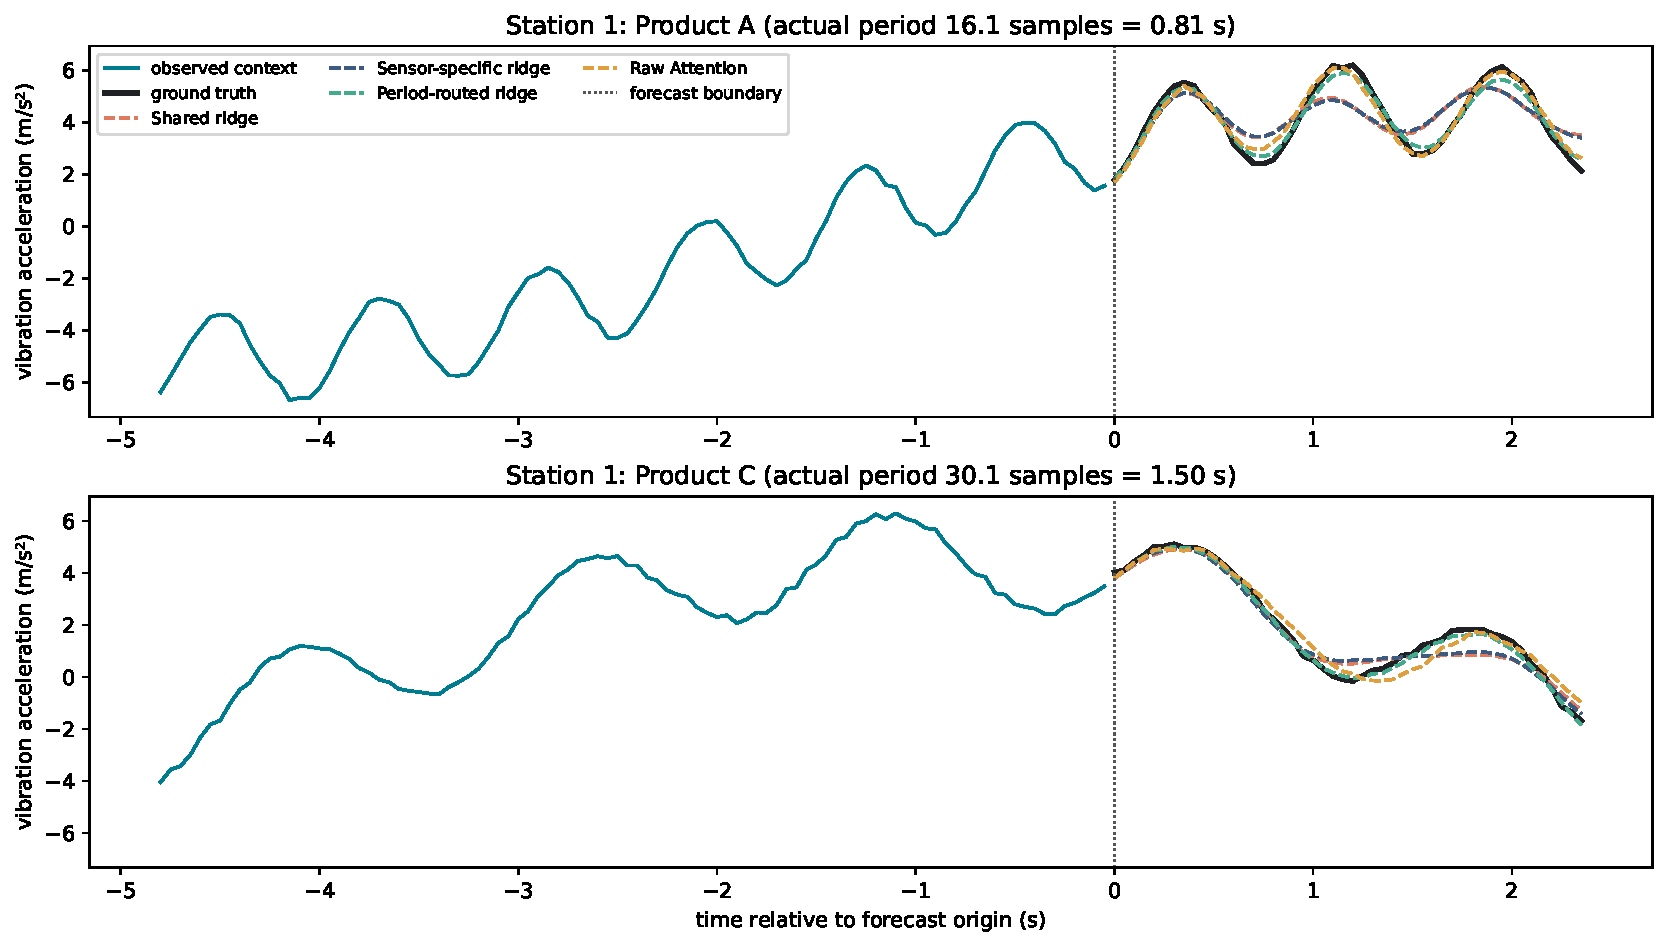
\includegraphics[width=0.9\linewidth]{../Figures/1.2-1.pdf}\caption*{Output 1.2 --- Station 1 under Product A ($P=16.1$) and Product C ($P=30.1$)}\end{figure}
\textbf{The fixed matrix $\hat W$ (Eq.~8) must compromise.} It applies one linear map whatever the pace. The Product A run ($P=16.1$) and the Product C run ($P=30.1$) need different phase advances over the 48-step horizon, but $\hat W$ contains no variable that selects between them. Least squares therefore averages the incompatible continuations. In Output 1.2 the shared-ridge forecast is damped (reduced amplitude), and its peaks drift out of phase with the truth as the lead time grows. The window RMSE shows this: shared ridge scores 0.779 (A) and 0.448 (C), while period-routed ridge scores 0.232 and 0.150.

\begin{figure}[H]\centering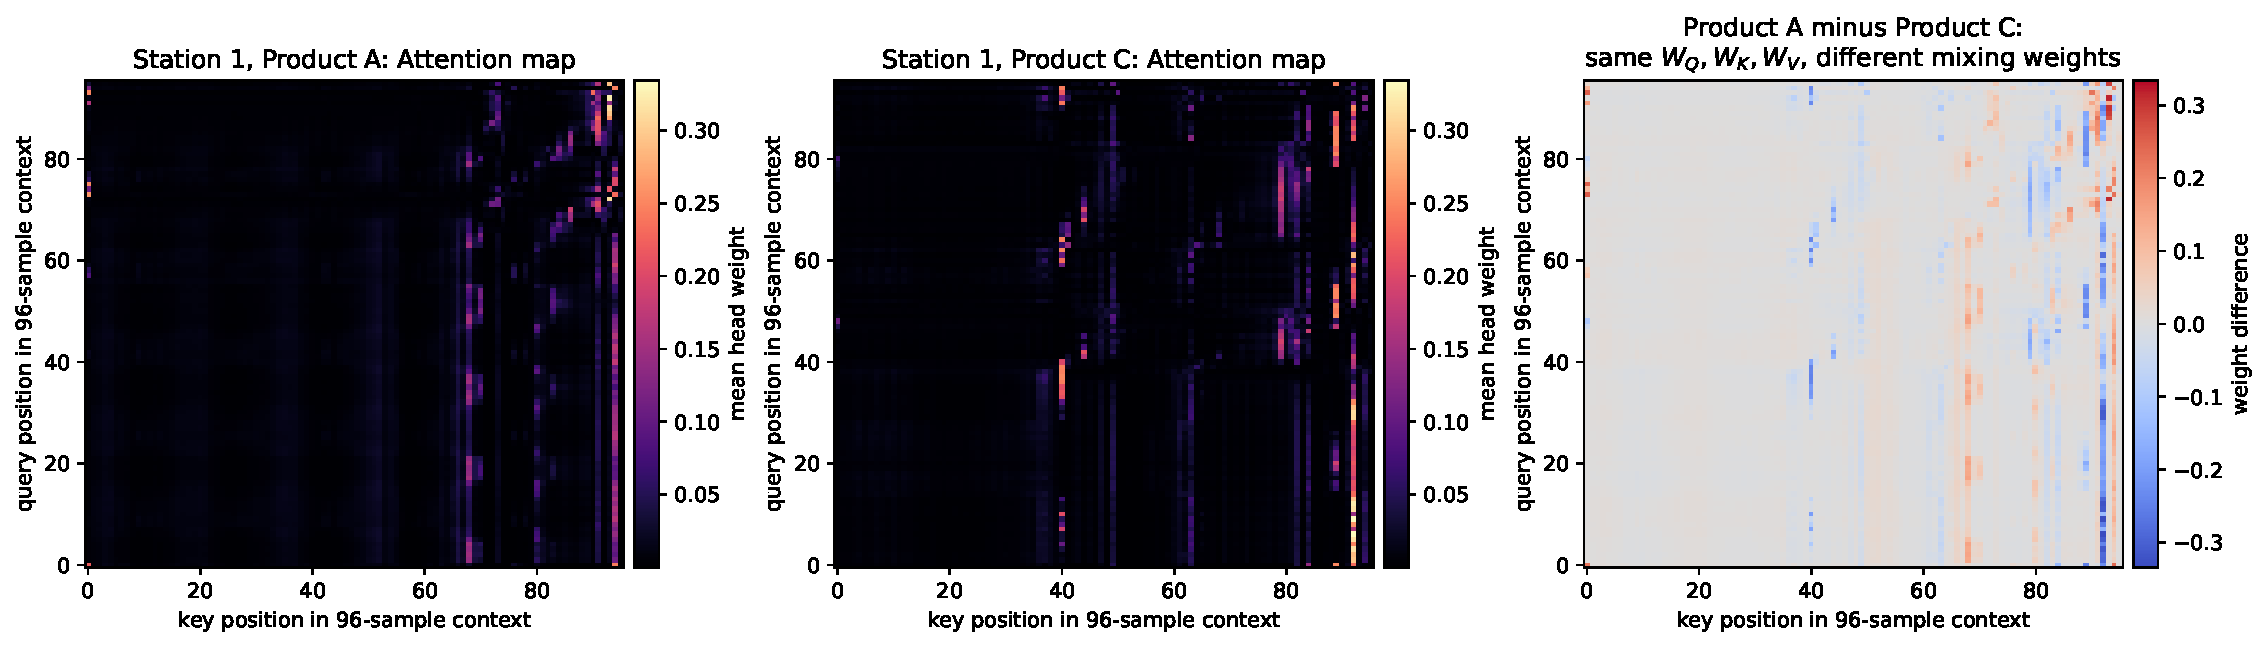
\includegraphics[width=0.9\linewidth]{../Figures/1.3-1.pdf}\caption*{Output 1.3 --- Attention weights for the two contexts and their difference}\end{figure}
\textbf{Attention builds its mixing rule from the context.} $W_Q,W_K,W_V$ are frozen after training and are identical for both windows. The scores $QK^\top$, however, are recomputed from each window's own features, so each context gets its own value-mixing matrix. The Product A and Product C maps differ by up to 0.334 in a single weight (mean absolute difference 0.013). Ridge, in contrast, applies the same $\hat W$ to every context. Output 1.3 only shows that the mixing weights depend on the input. It is not evidence that Attention has recovered the physical period.

\subsection*{Response 2: Series decomposition}
\texttt{SeriesDecomposition.forward} computes a centred moving average. It clamps the indices so that both ends replicate the nearest observed value. $T$ is this average and $S=x-T$, so $S+T=x$ exactly. The kernel-3 worked example (trend $[1.333, 2, 5, 6, 6.667]$) and the harness checks pass.
\begin{figure}[H]\centering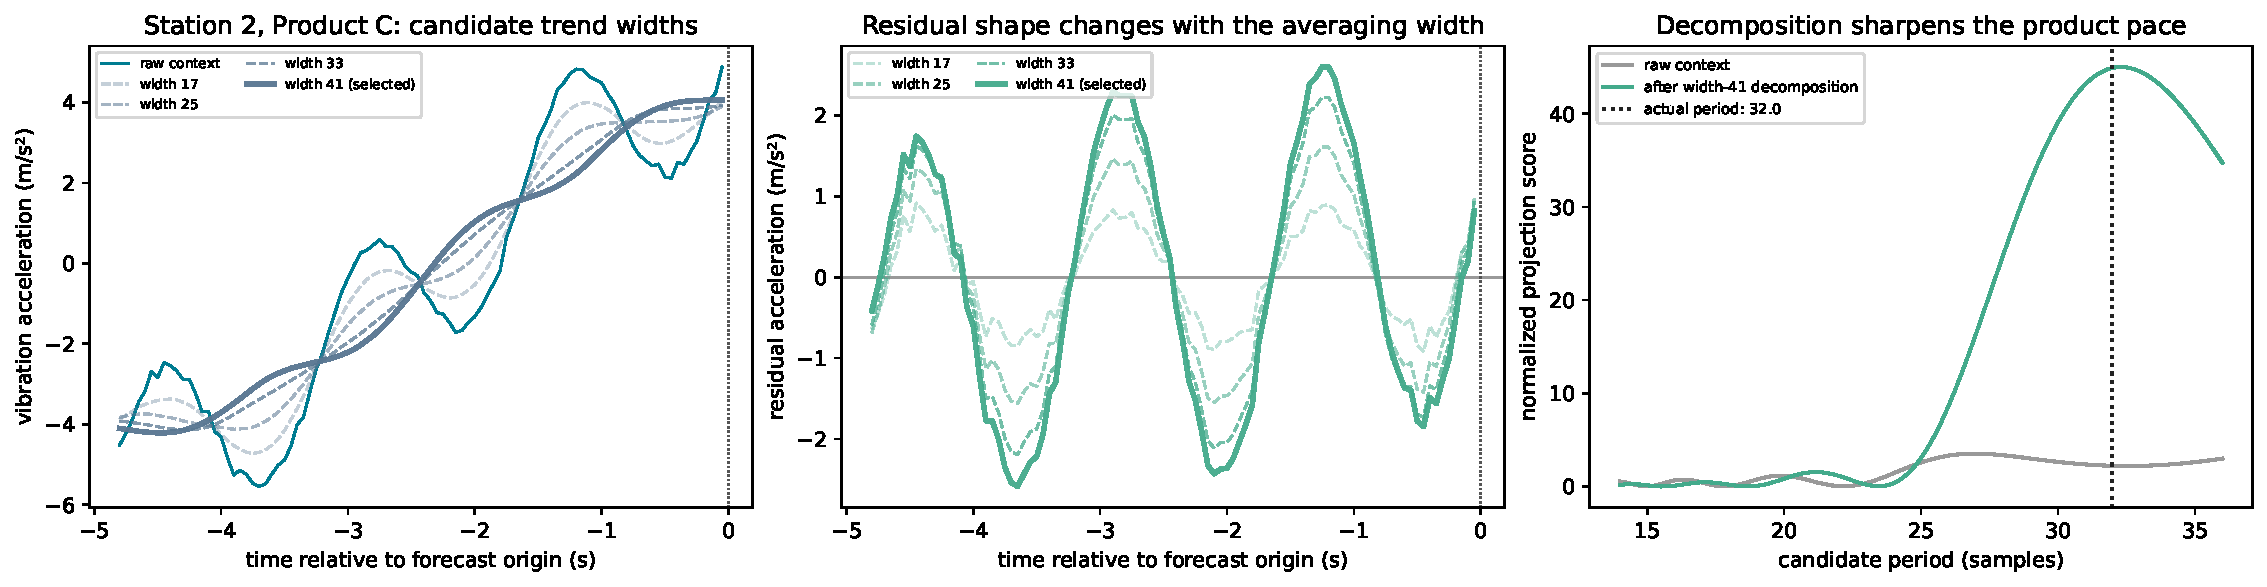
\includegraphics[width=0.85\linewidth]{../Figures/2.1-1.pdf}\caption*{Output 2.1 --- decomposition of one Station 2, Product C context ($P=32$) at widths 17--41}\end{figure}
\textbf{Selected width: $m=41$.} The study selects the width that gives the best oracle period recovery on the training data of Stations 1--3 (Output 2.2).
\begin{itemize}
\item \textbf{Visual change (Output 2.1).} At $m=17$ the trend still follows part of the vibration, so $S$ loses amplitude (residual std 0.58 m/s$^2$). As $m$ grows, $T$ becomes a smooth ramp and $S$ keeps the full cycle (std 1.01, 1.37 and 1.57 m/s$^2$ at 25, 33 and 41). After width-41 decomposition, the period score peaks sharply at the actual period of 32.
\item \textbf{Oracle diagnostic (Output 2.2, training windows).} Recovery within one sample is 0.687 on the raw context, then 0.980, 0.989, 0.993 and 0.998 at widths 17, 25, 33 and 41. There is a trade-off: the median period error is smallest at $m=25$ (0.12 samples, vs 0.22 at $m=41$). The selection rule counts hits within one sample, so $m=41$ wins.
\item \textbf{Ablation (Output 2.3, validation).} Raw Attention 0.466 $\to$ Attention + decomposition 0.310 on Est. ($-33\%$), and 0.679 $\to$ 0.455 on S4 ($-33\%$). Every product improves. The largest gain is S4, Product A (0.731 $\to$ 0.385), and the smallest is S4, Product B (0.617 $\to$ 0.518).
\end{itemize}
\begin{figure}[H]\centering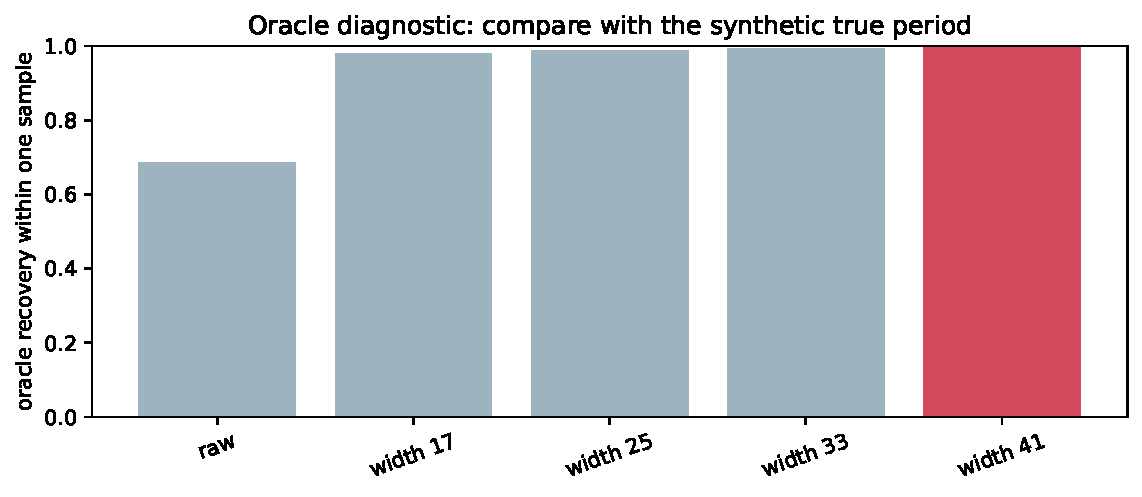
\includegraphics[width=0.75\linewidth]{../Figures/2.2-1.pdf}\caption*{Output 2.2 --- oracle period-recovery diagnostic (training data, Stations 1--3)}\end{figure}
\textbf{Why a moving average fits this world.} Drift (240-sample scale) and vibration (14--36 samples) are well separated in frequency. A moving average whose width spans at least one full cycle ($41>36$) cancels the vibration while still following the slow ramp, because $41\ll240$. It is therefore a cheap low-pass filter with its cutoff between the two components. The oracle diagnostic is a useful selector here because it scores what $S$ actually retains (is the true period recoverable from it?) instead of assuming that $S$ equals $s_i$. It uses only training windows from Stations 1--3, so neither S4 nor the validation and test regions influence $m$. The true period is available only in this synthetic world and is never given to the forecaster.
\begin{figure}[H]\centering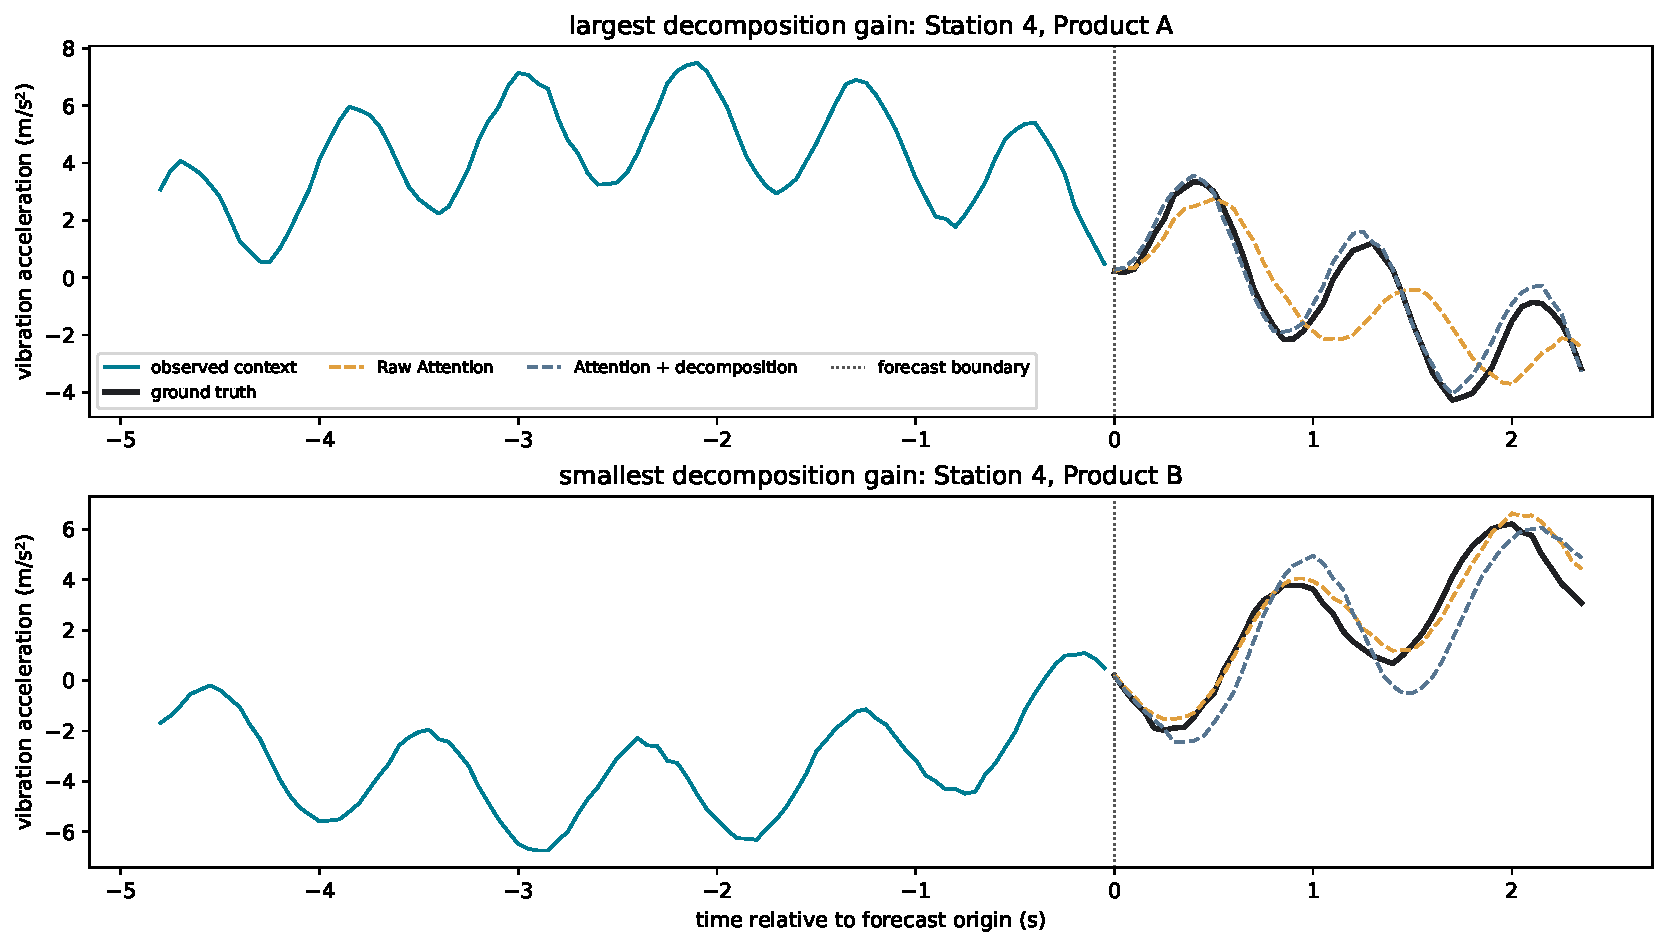
\includegraphics[width=0.75\linewidth]{../Figures/2.3-1.pdf}\caption*{Output 2.3 --- decomposition ablation (largest and smallest gain, S4)}\end{figure}
\textbf{Where it fails:} an abrupt level shift, such as a step in the calibration offset, is smeared into a ramp of width $m$, which leaks a fake trend into $S$ near the step. A wide kernel ($41\approx$ half the 96-sample context) also makes the replicated endpoints affect a large share of the window. \textbf{Alternative:} STL (LOESS) handles curved trends, but it assumes one known, fixed seasonal period. That assumption is wrong here, where pace changes from run to run.

\subsection*{Response 3: Temporal delay mixing}
\texttt{aggregate\_delays} (Eq.~6) builds the source index $(t-\tau_j)\bmod L$ for every example, delay and position. It gathers $v$ at those indices, weights the result by $\alpha_j$ (the same weights for all heads and features of that example), and sums over $j$. On the worked example ($v=[10,20,30,40]$, delays $[1,3]$, weights $[3/4,1/4]$) it returns $[35,15,25,25]$. Because $z_0=35$ (not 25), the shift reads $t-\tau$ in the correct direction. The FFT \texttt{delay\_scores} matches the direct calculation $[4,-4,4,-4]$ (Output 3.1).
\begin{figure}[H]\centering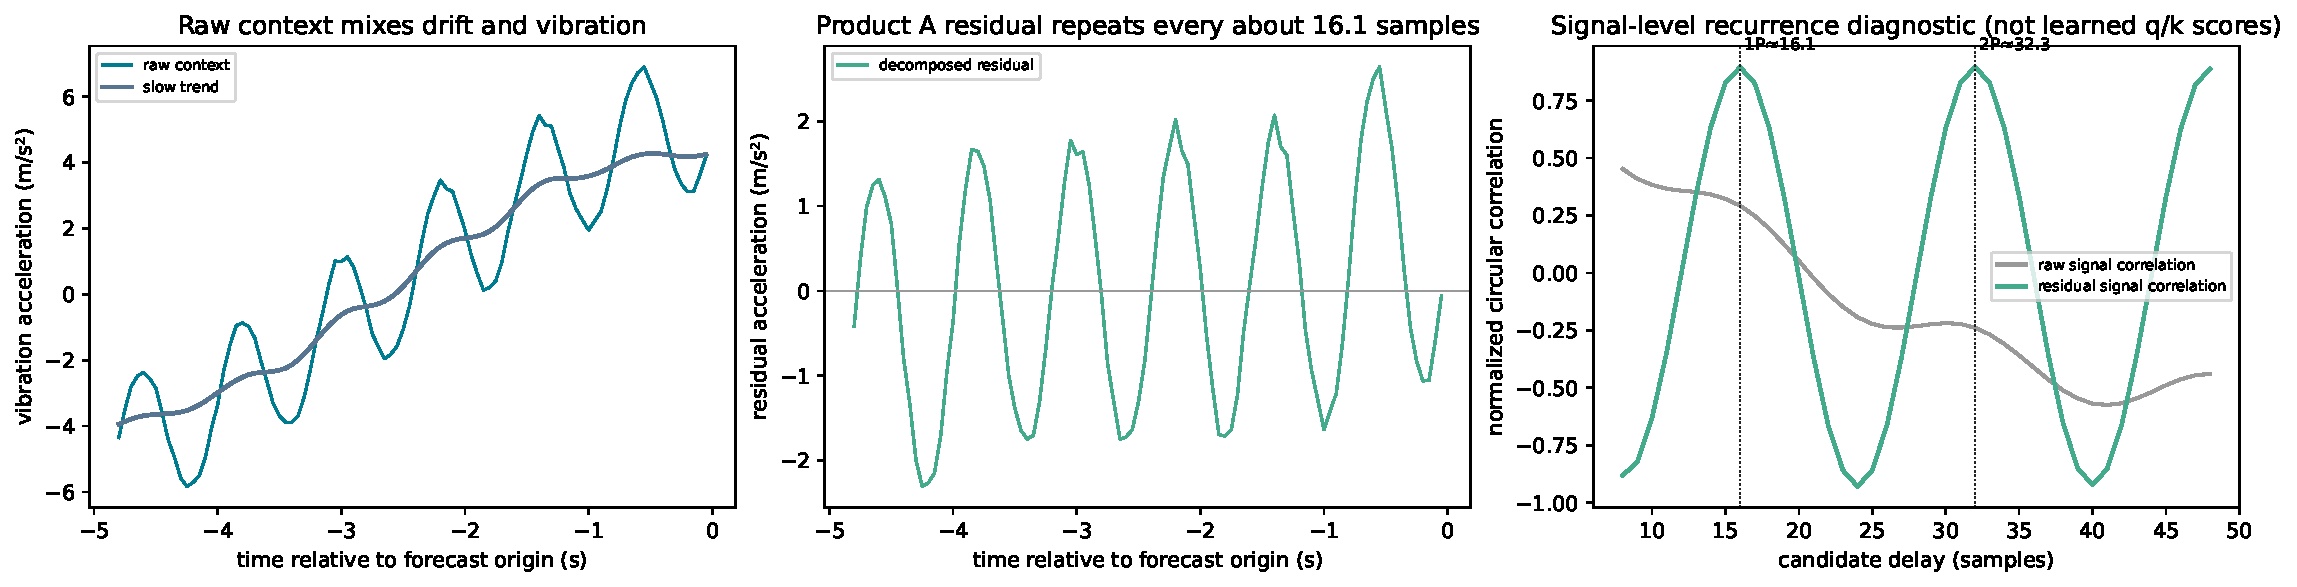
\includegraphics[width=0.85\linewidth]{../Figures/3.2-1.pdf}\caption*{Output 3.2 --- signal-level recurrence diagnostic, Station 2, Product A ($P\approx16.1$)}\end{figure}
\begin{itemize}
\item \textbf{Strongest lags:} the residual correlation peaks at lag 16 ($\approx P=16.1$, correlation 0.896) and at lag 32 ($\approx 2P=32.3$, correlation 0.897). A periodic signal matches itself at every integer multiple of $P$, so the second peak is the same recurrence one cycle further back. 
\item \textbf{Why decomposing first helps:} a ramp stays similar to itself after any shift. In the raw signal the correlation is therefore highest at the shortest lag ($\approx0.45$ at lag 8) and decays smoothly, with only a shallow shoulder near $P$ and no peak at $2P$. Once $T$ is removed, the curve swings between $\approx+0.9$ at $P$ and $2P$ and $\approx-0.9$ at the half-periods, and it rises again towards $3P\approx48$. The delays that matter then stand out, which is exactly the evidence the delay mixer selects with its top-$K$ step. This supports building the delay assumption into the mixer.
\item \textbf{Where the assumption is wrong:} an isolated transient, such as a single impact or shock, has no recurring displacement. Top-$K$ delay selection still picks $K=10$ lags, so the mixer either copies the shock forward at those lags, creating phantom repeats, or averages it away. Attention could instead have treated the transient as a one-off event.
\end{itemize}
\textit{Note: Output 3.2 is a correlation computed directly on the signal. It is not the trained mixer's learned q/k delay scores.}

\subsection*{Response 4: Compare designs and deploy}
\textbf{(a) Prediction (written before Output 4.1).} Decomposition should help most, because it removes the slow ramp before the mixer, so neither Attention nor the delay scores are dominated by drift.

\textbf{(b) Validation results} (Outputs 1.1, 4.1, 4.2).
\begin{table}[H]\centering\small
\begin{tabular}{lcccccr}\toprule
Model & Est. RMSE & Est. MSE & S4 RMSE & S4 MSE & Params & Fit time\\\midrule
Raw Attention & 0.466 & 0.217 & 0.679 & 0.461 & 368,368 & 158 s\\
Attention + decomposition & 0.310 & 0.096 & 0.455 & 0.207 & 373,024 & 455 s\\
Raw delay mixer & 0.215 & 0.046 & 0.341 & 0.116 & 368,370 & 239 s\\
Autoformer-inspired & 0.199 & 0.040 & 0.242 & 0.059 & 373,026 & 510 s\\\midrule
Shared ridge & 0.767 & 0.588 & 0.876 & 0.767 & 4,608 & $<$0.01 s\\
Sensor-specific ridge & 0.768 & 0.590 & n/a & n/a & 13,824 & $<$0.01 s\\
Period-routed ridge & \textbf{0.166} & \textbf{0.028} & \textbf{0.173} & \textbf{0.030} & 59,904 & $<$0.01 s\\\bottomrule
\end{tabular}\end{table}
\begin{figure}[H]\centering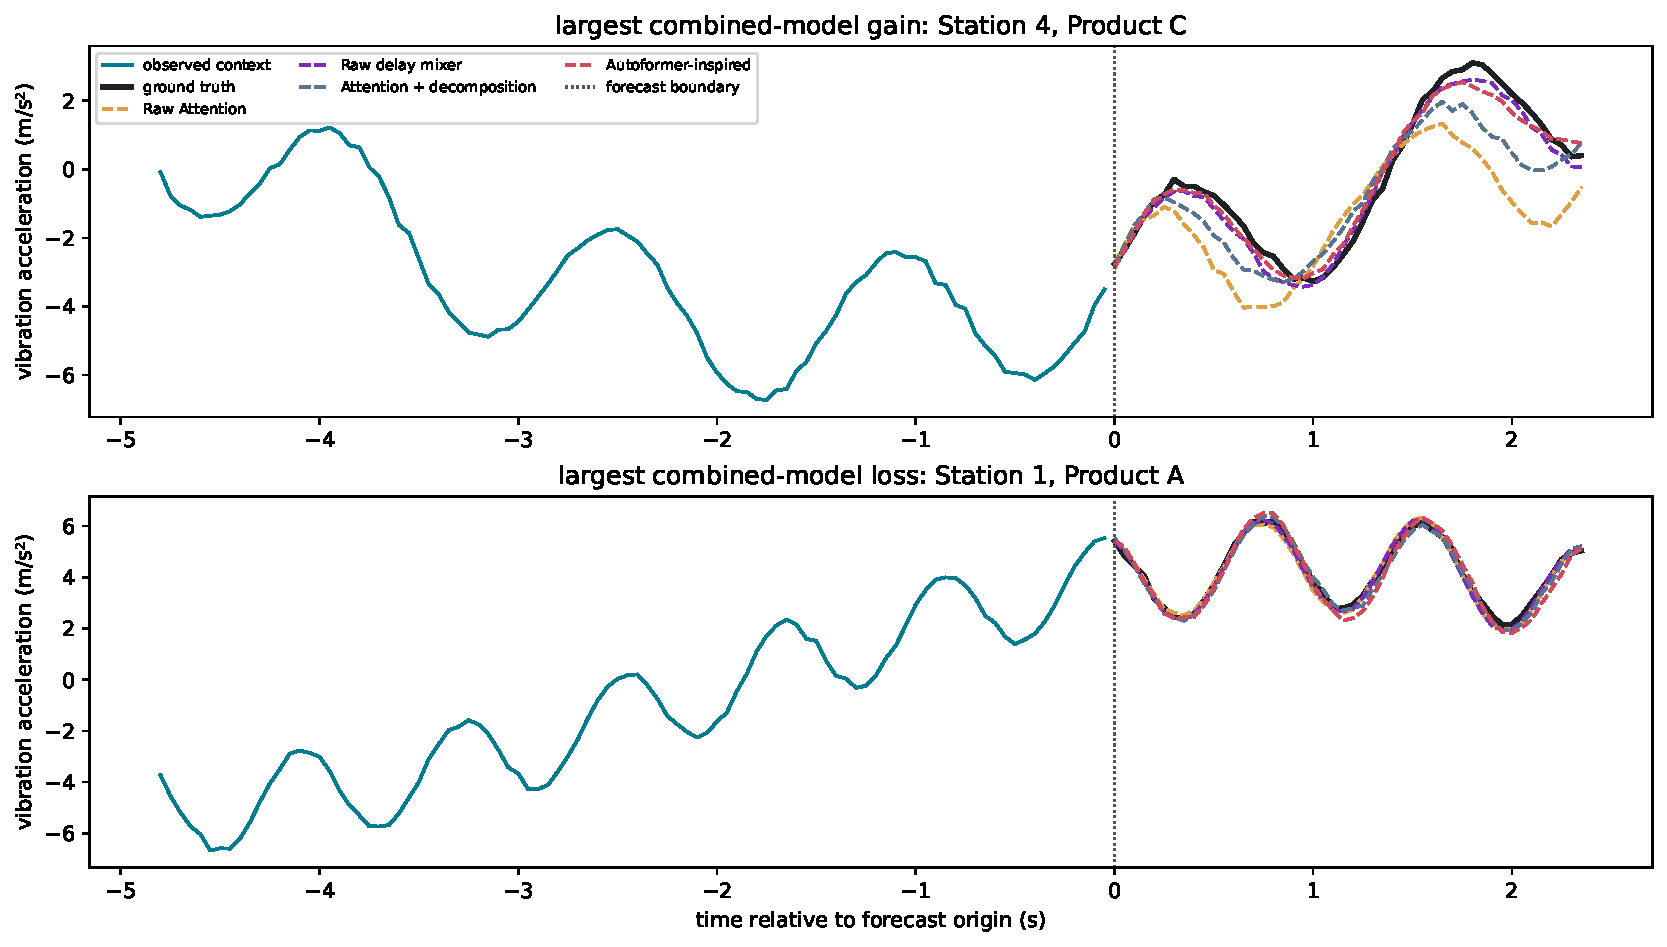
\includegraphics[width=0.85\linewidth]{../Figures/4.1-1.pdf}\caption*{Output 4.1 --- contrasting forecast cases (largest combined-model gain and loss)}\end{figure}
\begin{figure}[H]\centering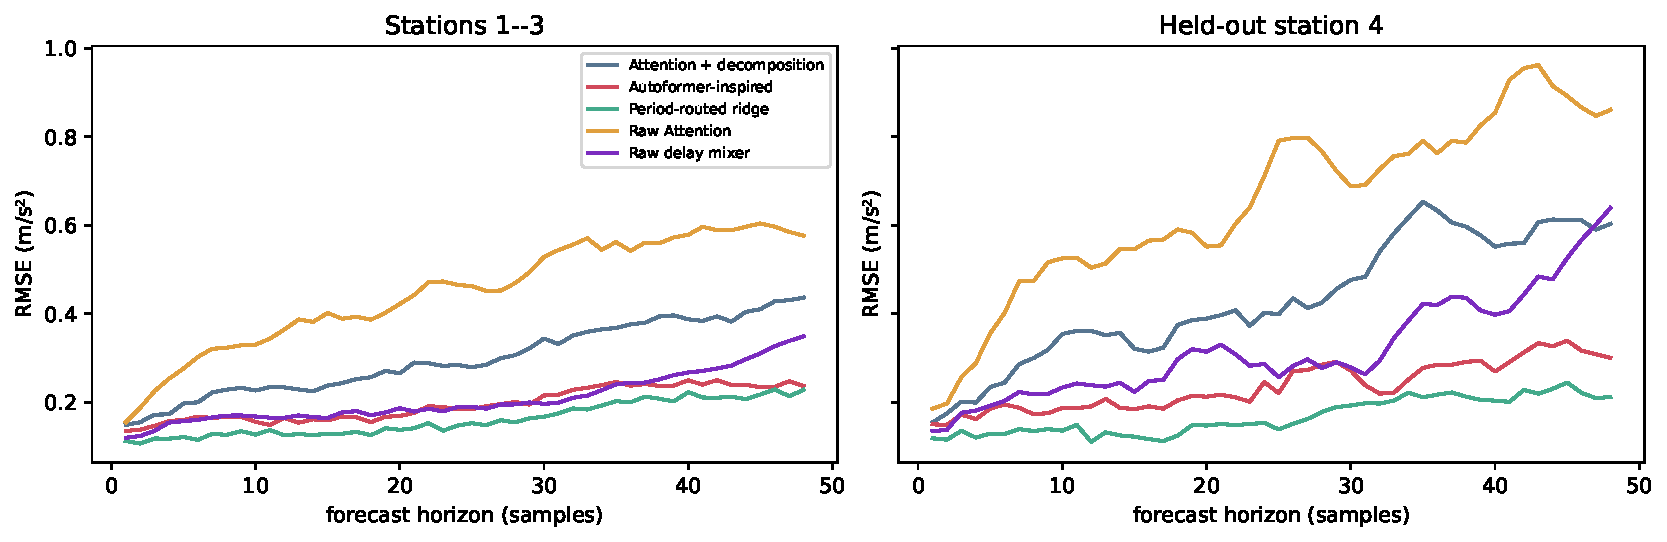
\includegraphics[width=0.75\linewidth]{../Figures/4.2-1.pdf}\caption*{Output 4.2 --- validation RMSE by forecast horizon}\end{figure}
\textbf{Interpretation} (validation; Est.\ / S4 RMSE reduction):
\begin{itemize}
\item \textbf{Delay switch:} $-54\%$ / $-50\%$ with the raw input, and $-36\%$ / $-47\%$ on top of decomposition.
\item \textbf{Decomposition switch:} $-33\%$ / $-33\%$ with Attention, but only $-7\%$ / $-29\%$ on top of the delay mixer.
\item \textbf{Overlap:} combined, $-57\%$ / $-64\%$. Gains are sub-additive (Est.: $0.251+0.156$ vs $0.267$ observed): both switches address the same drift-plus-repetition structure. Contrary to (a), delay mixing gives the larger gain. The combination is not uniformly better (Station 1, Product A is its largest loss, Output 4.1).
\item \textbf{Horizon:} error grows with lead time for all models (first vs last 12 steps): $\times$2.0--2.2 for both Attention models, $\times$1.5 / $\times$1.7 for Autoformer-inspired, and $\times$2.4 on S4 for the raw delay mixer. Period-routed ridge is lowest at all 48 steps.
\end{itemize}

\textbf{(c) Deployment} (chosen in the notebook before Output 4.3 was run).
\begin{itemize}
\item \textbf{Established stations: period-routed ridge.} It has the best validation RMSE/MSE (0.166 / 0.028 vs 0.199 / 0.040 for Autoformer-inspired), 6.2$\times$ fewer parameters, and fits instantly.
\item \textbf{Station 4: period-routed ridge.} It needs only the period estimated from S4's own context, not station identity (0.173 vs 0.242).
\item \textbf{Output 4.3 (test):} 0.161 (Est.) and 0.183 (S4), consistent with validation. The right inductive bias beats flexibility; Autoformer-inspired is the best \emph{learned} model.
\end{itemize}

\clearpage
\section*{Task 2 --- Leaderboard Challenge}

\subsection*{2.1 What the data says}
\begin{itemize}
\item \textbf{Sampling and horizon.} 43,824 rows is $5\times8{,}760$, so the series is almost certainly hourly over five years, and the horizon of 168 steps is one week. The mean by index mod 24 shows a clear daily cycle (Fig.~T2-1).
\item \textbf{Memory is short.} The autocorrelation is 0.97 at lag 1, 0.40 at lag 24, 0.16 at lag 48 and 0.03 at lag 168. The past alone says little about the second half of the week.
\item \textbf{Heavy tail.} Mean 98, median 73, 99th percentile 418, maximum 994. RMSE is dominated by the rare high episodes.
\item \textbf{The optional file is future-known weather.} It has 6 continuous and 4 mutually exclusive binary columns: two temperature-like columns (A, B), pressure (C), a cumulative wind speed that restarts when the binary state changes (D), and two rare cumulative counts (E, F). The four flags behave like a wind-direction indicator. The target mean under each flag is G 90, H 70, I 110, J 125: flag H clears the air, while J (stagnant conditions) lets it accumulate.
\end{itemize}
\begin{figure}[H]\centering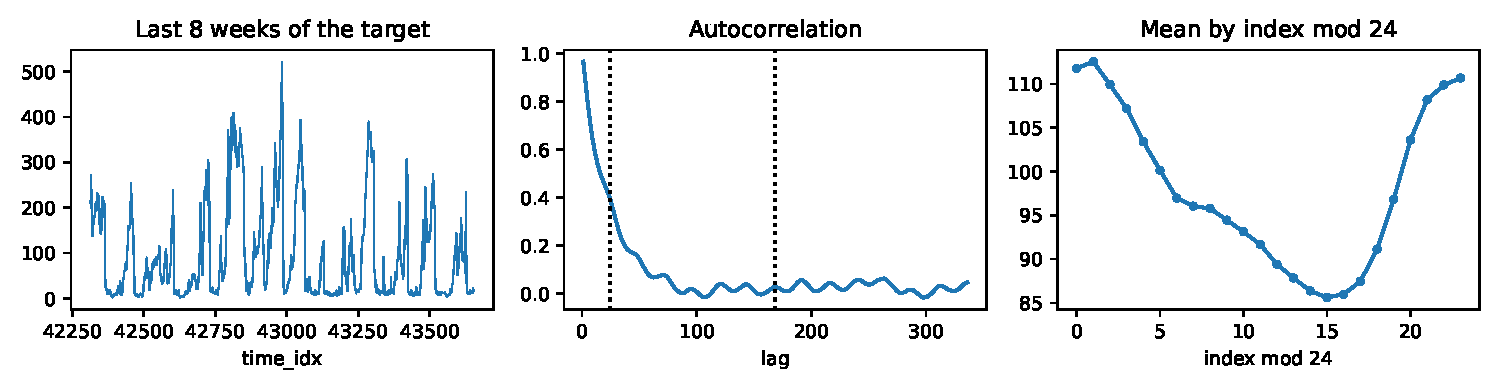
\includegraphics[width=\linewidth]{../Figures/T2-1_data.pdf}\caption*{Fig.~T2-1 --- last 8 weeks, autocorrelation, daily profile.}\end{figure}

\subsection*{2.2 Validation protocol (fixed before any v3 study)}
With 5 leaderboard attempts, the leaderboard cannot be a tuning signal, so every decision below uses my own chronological validation.
\begin{itemize}
\item \textbf{Two folds}, each trained only on rows before it:
  \begin{itemize}
  \item \emph{winter}: rows 33,600--36,480. If the series starts on 1 January, this is November--February of the previous winter. The hidden week is then the last week of December, so this fold matches its season.
  \item \emph{recent}: the last 16 weeks of the history.
  \end{itemize}
\item \textbf{Scoring.} A forecast starts every 24 steps, giving 220 forecasts of 168 steps in total. All lead times are scored on the raw scale with RMSE, MAE and sMAPE.
\item \textbf{Seeds.} Every option is trained with 3 seeds. I report the per-seed mean $\pm$ std and the RMSE of the 3-seed average.
\item \textbf{Selection rule.} The option with the lowest mean per-seed RMSE, pooled over both folds, wins.
\end{itemize}
\emph{Why two folds?} A single 168-step validation block is noisy: the gap between two designs can be smaller than week-to-week variation, so one block is a weak basis for model selection.

\subsection*{2.3 Model: an encoder--decoder Autoformer}
I wrote the model from scratch, following Wu et al.\ (2021), \S\S3.1--3.2, and reusing my own Task 1 decomposition and delay-aggregation code. It contains both required mechanisms:
\begin{itemize}
\item \textbf{Series decomposition (progressive).} A moving average (kernel 25, endpoint replication) splits the input into seasonal and trend parts. The same split is applied again after \emph{every} sub-layer of the encoder and decoder. The trend pieces removed in the decoder are projected and accumulated into the trend path.
\item \textbf{Auto-Correlation.}
  \begin{itemize}
  \item Delay scores $R(\tau)=\sum_t q_t k_{t-\tau}$ are computed by FFT in $O(L\log L)$, and the top $k=\lfloor 2\ln L\rfloor$ delays are kept: $k=9$ in the encoder ($L=96$) and $k=10$ in the decoder ($L=48+168=216$).
  \item Weights: $\alpha=\mathrm{softmax}(R/\vartheta)$ with a learned temperature $\vartheta$.
  \item Aggregation: $z_t=\sum_j \alpha_j v_{t-\tau_j}$.
  \item The decoder uses it twice: on itself, and across to the encoder output.
  \item There is no dot-product attention anywhere in the model.
  \end{itemize}
\item \textbf{Lengths and size.}
  \begin{itemize}
  \item Context $L=96$ (memory is short, \S2.1); decoder input = last 48 context steps + 168 placeholder steps; \texttt{pred\_len}$=168$.
  \item $d_{model}=16$, one encoder layer, one decoder layer: 9,159 parameters.
  \end{itemize}
\item \textbf{Normalisation.} Global standardisation of the raw target, fitted on the training rows only. I did not use window-relative normalisation, because the absolute level is what the weather explains.
\end{itemize}
\emph{Two design changes of my own:}
\begin{enumerate}
\item \textbf{Covariate embedding.} Covariates enter through a 2-layer MLP followed by a centred depthwise temporal convolution (kernel 5), so each step also sees the weather of nearby hours. This was not ablated on its own; it is part of every covariate row in S1.
\item \textbf{Trend start.} The decoder trend starts at the context mean \emph{plus a linear function of the covariates}, instead of the paper's context mean alone. Over a whole week the level is set by the weather, not by the past window. This is tested in S2.
\end{enumerate}

\subsection*{2.4 Where the optional data enters, and what it did}
The covariates for the horizon are known at forecast time, so they enter the \textbf{decoder} at all 168 forecast steps. Past covariates enter the encoder.

\textbf{Engineered features} (all backward-looking, scaled on training rows only):
\begin{itemize}
\item hourly wind speed, recovered from the cumulative column D (it restarts when the direction flag changes);
\item that wind speed split by direction flag, each smoothed with an exponential moving average with half-lives of 6, 24 and 72 h (pollution builds up and is flushed out gradually);
\item the A$-$B gap (dew-point-depression style humidity proxy), the share of flag-J (calm) hours, and the 24-h change in C;
\item sin/cos of the daily (24) and yearly (8,766) position, to recover the cycles without timestamps.
\end{itemize}
This gives 34 inputs per step. The four index-derived sin/cos terms do not come from the optional file, so they are kept in every S1 row, including ``none''.

\begin{table}[H]\centering\small
\caption*{Study S1 --- ablation of the optional file (final architecture, 3 seeds, both folds)}
\begin{tabular}{lccccc}\toprule
Optional data & RMSE / seed & 3-seed avg & winter & recent & MAE / sMAPE\\\midrule
none & 142.6 $\pm$ 3.7 & 141.9 & 142.6 & 141.1 & 120.6 / 95.0\%\\
raw file, past only (horizon masked) & 125.9 $\pm$ 0.5 & 124.7 & 127.7 & 121.3 & 104.4 / 90.2\%\\
raw file, past + future & 85.9 $\pm$ 11.1 & 81.0 & 81.1 & 80.9 & 62.4 / 68.6\%\\
\textbf{engineered, past + future} & \textbf{81.8 $\pm$ 9.8} & \textbf{76.8} & 75.8 & 77.8 & 59.3 / 66.2\%\\\bottomrule
\end{tabular}\end{table}
\begin{figure}[H]\centering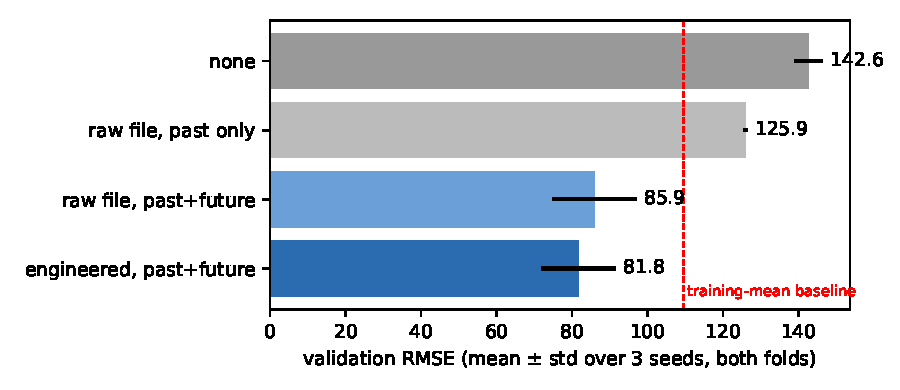
\includegraphics[width=0.6\linewidth]{../Figures/T2-2_ablation.pdf}\caption*{Fig.~T2-2 --- S1 ablation; dashed line = training-mean baseline.}\end{figure}
\textbf{Finding.} The optional file helps a lot, but only its \emph{horizon} part does: past-only covariates help a little (142.6 $\to$ 125.9), while adding the horizon covariates cuts the error by a further 32\% (125.9 $\to$ 85.9). The engineered features then gain another 4.1 (85.9 $\to$ 81.8). Both target-only and past-only models are worse than the training-mean baseline (116.3 / 102.8 on the two folds). Without future weather, the short memory leaves nothing to predict a week ahead, and the model fits noise.

\subsection*{2.5 Design studies (each starts from the winner of the previous one)}
\begin{table}[H]\centering\small
\begin{tabular}{llccc}\toprule
Study & Option & RMSE / seed & 3-seed avg & chosen\\\midrule
S2 trend start & context mean (paper) & 83.9 $\pm$ 3.1 & 80.7 & \\
 & mean + linear(covariates) & 81.8 $\pm$ 9.8 & 76.8 & \checkmark\\\midrule
S3 target & raw & 81.8 $\pm$ 9.8 & 76.8 & \checkmark\\
 & log1p & 163.2 $\pm$ 72.6 & 128.5 & \\
 & average of raw and log models & 107.2 $\pm$ 37.7 & 93.3 & \\\midrule
S4/S5 epochs & 1 & 77.8 $\pm$ 0.3 & 75.4 & \\
 & 2 & \textbf{77.1 $\pm$ 1.0} & \textbf{74.0} & \checkmark\\
 & 3 / 4 / 6 & 82.7 / 81.8 / 89.3 & 79.5 / 76.8 / 86.0 & \\\midrule
S6 width & $d=8$ / 16 / 32 & 77.2 / \textbf{77.1} / 81.7 & 72.9 / 74.0 / 72.2 & $d=16$\\\midrule
S7 dropout & 0.1 / 0.3 & \textbf{77.1} / 88.9 & 74.0 / 73.2 & 0.1\\\bottomrule
\end{tabular}\end{table}
\begin{itemize}
\item \textbf{Trend start.} The covariate trend wins on the mean (81.8 vs 83.9), and by 4 points in the 3-seed average.
\item \textbf{Target scale.} The log target is unstable: one seed exploded, because \texttt{expm1} amplifies any error at high values. The raw target matches the RMSE that is scored.
\item \textbf{Epochs.} Two epochs are best, and the model overfits beyond that (Fig.~T2-3). One epoch is the most stable ($\pm0.3$) but under-fits the winter fold (79.2).
\item \textbf{Width and dropout.} $d=8$ and $d=16$ are tied per seed. $d=32$ and dropout 0.3 average slightly better but have 5 and 7 times the seed spread, which I do not trust with 5 attempts.
\end{itemize}
\begin{figure}[H]\centering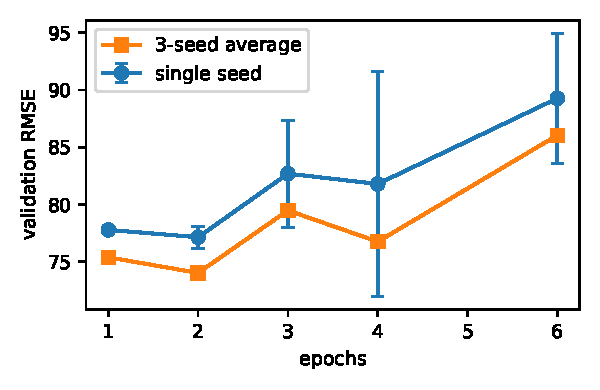
\includegraphics[width=0.45\linewidth]{../Figures/T2-3_epochs.pdf}\caption*{Fig.~T2-3 --- validation RMSE vs epochs.}\end{figure}

\subsection*{2.6 Final model, validation behaviour and limits}
\textbf{Configuration:} context 96, $d=16$, 1+1 layers, kernel 25, $k=\lfloor 2\ln L\rfloor$ (9 / 10), dropout 0.1, raw target, engineered future covariates, covariate trend start, 2 epochs.\\
\textbf{Training:} AdamW (lr $3\cdot10^{-3}$, weight decay $10^{-3}$), 10\% warm-up then cosine decay, batch 256, gradient clipping at 1.0, MSE loss, every window used (stride 1).\\
\textbf{Validation of the 3-seed average:}
\begin{itemize}
\item winter fold: RMSE 74.4, MAE 53.3, sMAPE 60.5\%;
\item recent fold: RMSE 73.6, MAE 57.1, sMAPE 66.8\%.
\end{itemize}
\begin{figure}[H]\centering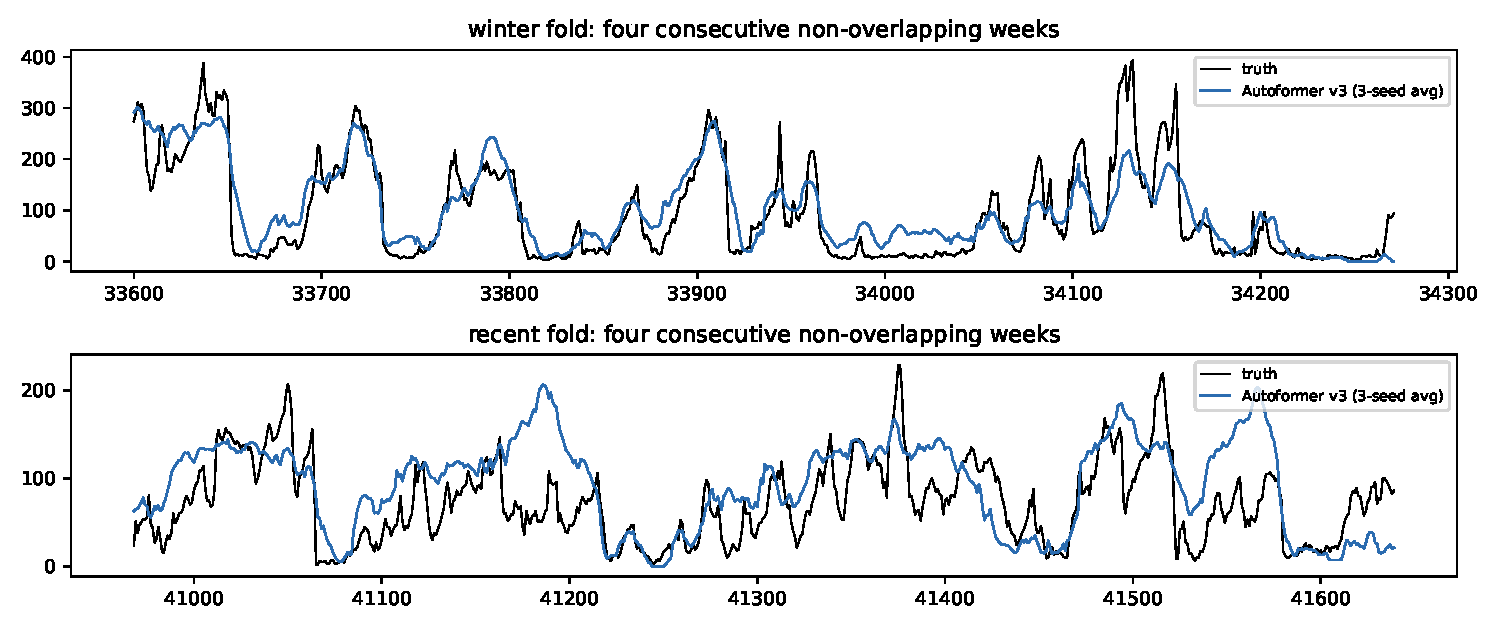
\includegraphics[width=\linewidth]{../Figures/T2-4_val_forecasts.pdf}\caption*{Fig.~T2-4 --- validation forecasts vs truth (four consecutive weeks per fold).}\end{figure}
\begin{figure}[H]\centering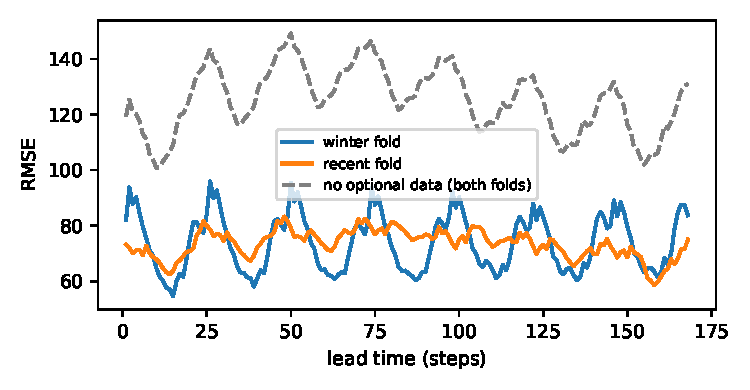
\includegraphics[width=0.5\linewidth]{../Figures/T2-5_lead_time.pdf}\caption*{Fig.~T2-5 --- RMSE by lead time.}\end{figure}
\begin{itemize}
\item \textbf{Flat error across the horizon} (Fig.~T2-5): about 73 in the first 24 steps and 75 in the last 24 (winter). The forecast is driven by the known future weather rather than by past values, so it does not drift away over the week.
\item \textbf{Weakness: the peaks.} The top 10\% of true values (above 282) carry 32\% of the squared error and are under-forecast by 103 on average, while the remaining values are over-forecast by 30. Under squared loss the model shrinks toward the conditional mean. This is also why sMAPE stays near 60\%.
\end{itemize}

\textbf{Submission.} 5 seeds, refit on the \emph{full} history for 2 epochs each, then averaged. The refit includes the newest weeks the forecast starts from. In validation, averaging seeds improved RMSE by 3 (77.1 $\to$ 74.0).
\begin{itemize}
\item $P = 5\times 9{,}159 = \mathbf{45{,}795}$ and $E = 5\times 2=\mathbf{10}$ (fixed schedule, no early stopping).
\item The size and epoch penalties together add only about 0.005 to the score.
\item Both numbers are reproducible with \texttt{python q2\_v3.py final 5}.
\end{itemize}
\begin{figure}[H]\centering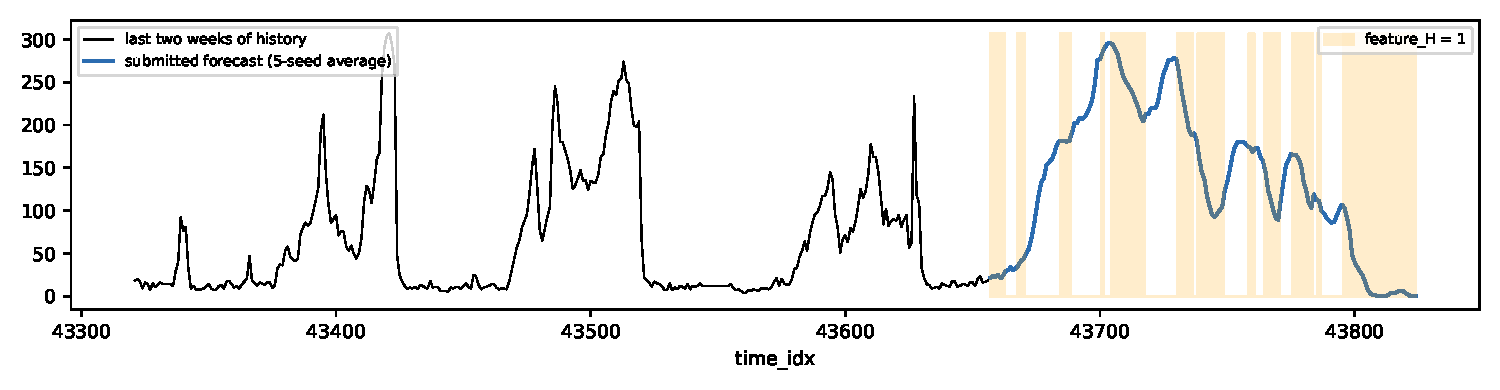
\includegraphics[width=\linewidth]{../Figures/T2-6_forecast.pdf}\caption*{Fig.~T2-6 --- submitted 168-step forecast (time\_idx 43657--43824); shaded: flag H.}\end{figure}

\textbf{Leaderboard result for this submission:} RMSE 68.34, MAE 51.54 and sMAPE 61.91\%, for a score of 68.341 with $P=45{,}795$ and $E=10$. The penalty terms add only about 0.005. The RMSE is a little better than the two-fold validation estimate (74.0); one 168-step week is a single noisy block, so I treat the leaderboard as a confirmation of the validation estimate, not as a tuning signal.

\subsection*{2.7 Reflection questions}
\begin{description}
\item[Q2.1 Auto-Correlation vs self-attention.]
\begin{itemize}
\item \emph{Where Auto-Correlation wins:} signals that repeat with a stable period, possibly several (e.g.\ a daily load cycle). Every pair at the same lag is related for the same reason, so scoring $L$ lags is better than scoring $L^2$ pairs.
\item \emph{What it discards:} content-specific links that do not repeat at a fixed lag, such as a one-off spike or a regime-dependent event. It aggregates whole shifted sequences and loses point-wise matches.
\item \emph{Drifting period:} a fixed set of lags blurs the forecast, while attention can still match individual similar points. Here the daily lag-24 structure is weak (ACF 0.40), which is why the covariates carry most of the signal.
\end{itemize}

\item[Q2.2 Moving-average trend.]
\begin{itemize}
\item \emph{What it assumes:} the trend is locally linear over the kernel, and the seasonal part averages to zero over $m$ steps.
\item \emph{At the boundaries:} endpoint replication flattens the trend near the window's end, which is exactly where the forecast starts.
\item \emph{Curvature and level shifts:} curvature is shaved off, and an abrupt level shift is smeared into a ramp of width $m$. Both matter for this heavy-tailed series.
\item \emph{Alternative:} a robust local-linear (LOESS or Hodrick--Prescott) trend. It follows curvature and the endpoint slope, but costs more computation and introduces a smoothing parameter that is harder to tune.
\end{itemize}

\item[Q2.3 Progressive vs one-shot decomposition.]
\begin{itemize}
\item \emph{What it buys:} each Auto-Correlation and FFN layer can re-introduce slow structure. Removing it after every sub-layer keeps the seasonal stream clean for the next delay scoring, and lets the decoder build the trend from learned pieces.
\item \emph{When it hurts:} if the useful signal is the level itself (as here, where the weather sets it), repeated smoothing removes it from the seasonal stream. A 24-h pollution episode is close to the kernel width (25), so it gets split between the two streams. My covariate trend start partly compensates for this.
\end{itemize}

\item[Q2.4 $k=c\log L$.]
\begin{itemize}
\item \emph{Small $k$} commits to few lags: low variance if they are right, large error if they are wrong.
\item \emph{Large $k$} hedges (like averaging) but admits noisy lags and drifts toward plain smoothing.
\item \emph{$\log L$ is convenient rather than principled:} it keeps the cost at $O(L\log L)$. Ideally $k$ should be a little larger than the number of real periodicities and their harmonics; with $L=96$, $k=9$ covers 24, 48, 72 and their neighbours.
\end{itemize}

\item[Q2.5 One-shot vs autoregressive.]
\begin{itemize}
\item \emph{Autoregressive} forecasting compounds its own errors and suffers exposure bias (it is trained on true inputs but run on its predictions). Its errors are strongly correlated along the horizon.
\item \emph{One-shot} forecasting (used here) has no feedback loop, and its error stays flat over 168 steps (Fig.~T2-5). It may produce less coherent paths.
\item \emph{When to prefer each:} autoregressive suits short horizons with smooth, low-noise dynamics. One-shot is better as the horizon and noise grow, especially when future covariates exist.
\end{itemize}

\item[Q2.6 Window normalisation.]
\begin{itemize}
\item \emph{What it destroys:} the absolute level and scale of each window.
\item \emph{Where it helps:} series whose level wanders while the shape repeats (sales with drifting demand).
\item \emph{Where it loses something essential:} when the level itself is predictable from outside, as here. "Calm, humid, southerly wind" means a high absolute value whatever the last window's mean was; stripping each window's mean throws that signal away.
\end{itemize}

\item[Q2.7 Past-only vs future-known covariates.]
\begin{itemize}
\item \emph{Where they enter:} past-only covariates belong in the encoder. Future-known ones should also enter the decoder at each forecast step, which is where the 32\% gain in S1 came from.
\item \emph{Useful only when future-known:} forecast wind speed or direction. It explains the level at the same hour but has little lagged effect beyond a day.
\item \emph{Equally useful in both:} the hour of day, which can always be computed.
\end{itemize}

\item[Q2.8 No timestamps.]
\begin{itemize}
\item \emph{What is lost:} holidays, weekdays and calendar season.
\item \emph{How to recover periodic structure:} from the index, through the autocorrelation/FFT peak (24) and the yearly position ($\approx$8,766 steps), encoded as sin/cos.
\item \emph{What this assumes:} uniform sampling (guaranteed by the handout) and that the series starts at a known phase. Otherwise only relative phase is identified.
\end{itemize}

\item[Q2.9 Structural models vs decomposition Transformers.]
\begin{itemize}
\item \emph{When structural models win:} short series, low signal-to-noise, and one dominant regular cycle. Their few parameters cannot overfit.
\item \emph{When Transformers win:} long series (tens of thousands of points), nonlinear covariate effects and several interacting regimes.
\item \emph{How to decide before training:} check the series length per parameter, the strength of the seasonal ACF peaks, and how much a linear covariate regression already explains. Here the series is long and nonlinear in the covariates, but it is noisy, so I kept the model tiny (9K parameters, 2 epochs).
\end{itemize}
\end{description}


\section*{References and attribution}
\begin{itemize}
\item Wu, Xu, Wang, Long (2021). \emph{Autoformer: Decomposition Transformers with Auto-Correlation for Long-Term Series Forecasting}, \S\S3.1--3.2. The architecture follows this paper; the layer layout follows the authors' public code (\url{https://github.com/thuml/Autoformer}). My code is written from scratch.
\item Vaswani et al.\ (2017); Zeng et al.\ (2023); Hyndman \& Athanasopoulos, \emph{Forecasting: Principles and Practice}.
\end{itemize}

\section*{Appendix: Generative AI disclosure}
I used \textbf{Claude (Anthropic)} in the Cursor IDE for limited debugging help and for polishing wording. The experimental design, model choices, coding of the main pipeline, running of all studies, and the interpretation of results are my own. I checked every reported number against the notebook outputs and logs, and I can explain every component of the submitted code.

\textbf{Prompt record (required by the course AI policy):}
\begin{enumerate}
\item \textbf{Prompt:} ``I already have a centred moving-average sketch for Eq.~3, but the endpoint padding is off and the worked example gives trend $[1.333,2,5,6,6.667]$. Where should the clamp sit, and is my circular shift for Eq.~6 indexing $t-\tau_j$ correctly?''\\
\textbf{Output:} a short note on clamping the pad indices and using \texttt{gather} for the delayed values.\\
\textbf{My edits:} kept my own structure, applied the clamp/\texttt{gather} fix, verified both worked examples ($z_0=35$), ran the full preset, and selected $m=41$ from Outputs 2.1/2.2.
\item \textbf{Prompt:} ``My Task~2 single-block validation looks optimistic relative to held-out behaviour. Does that sound like leakage, a bad fold, or weak use of the horizon covariates?''\\
\textbf{Output:} a short diagnosis pointing at single-block validation and weak horizon-covariate use, plus a suggestion to try two chronological folds with multiple seeds.\\
\textbf{My edits:} I designed the winter/recent folds and the selection rule (lowest mean per-seed RMSE) myself.
\item \textbf{Prompt:} ``I am wiring future covariates into my Autoformer decoder. Does feeding them only in the encoder look wrong, and is a small MLP on the covariate channels a reasonable place to start?''\\
\textbf{Output:} confirmed that future-known covariates should also enter the decoder, and that a small MLP is a common first choice.\\
\textbf{My edits:} wrote \texttt{q2\_v3\_model.py}/\texttt{q2\_v3.py} myself (reusing my Task~1 decomposition and delay code), engineered the features (recovered wind speed, EWMA memory, humidity proxy), chose the covariate trend start, ran the multi-seed studies, recounted $P$ and $E$, and checked time\_idx order before submitting.
\item \textbf{Prompt:} ``Can you tighten the wording of this reflection paragraph and suggest a matplotlib layout for four small panels? I will paste my own numbers and captions.''\\
\textbf{Output:} shorter phrasing and a 2$\times$2 subplot sketch.\\
\textbf{My edits:} rewrote every response in my own words, built the figures from my study logs, and checked every table against the logs.
\item \textbf{Prompt:} ``Please skim this draft against the handout checklist and flag any number that looks stale relative to the notebook outputs I pasted.''\\
\textbf{Output:} a short list of likely stale Task~1 figures.\\
\textbf{My edits:} corrected those sections from the re-executed notebook and kept period-routed ridge as the deployment choice (best on validation).
\end{enumerate}
\end{document}
